
\subsection*{Task} % (fold)
\label{sub:Task}
When a bug report is submitted, someone has to look at it and determine which component it affects and assigned an appropriate label. Currently it is done manually by one of the maintainers. We wondered if it's possible to use data mining to automatically classify new bugs by component.

\begin{figure}[!htp]
\begin{center} 
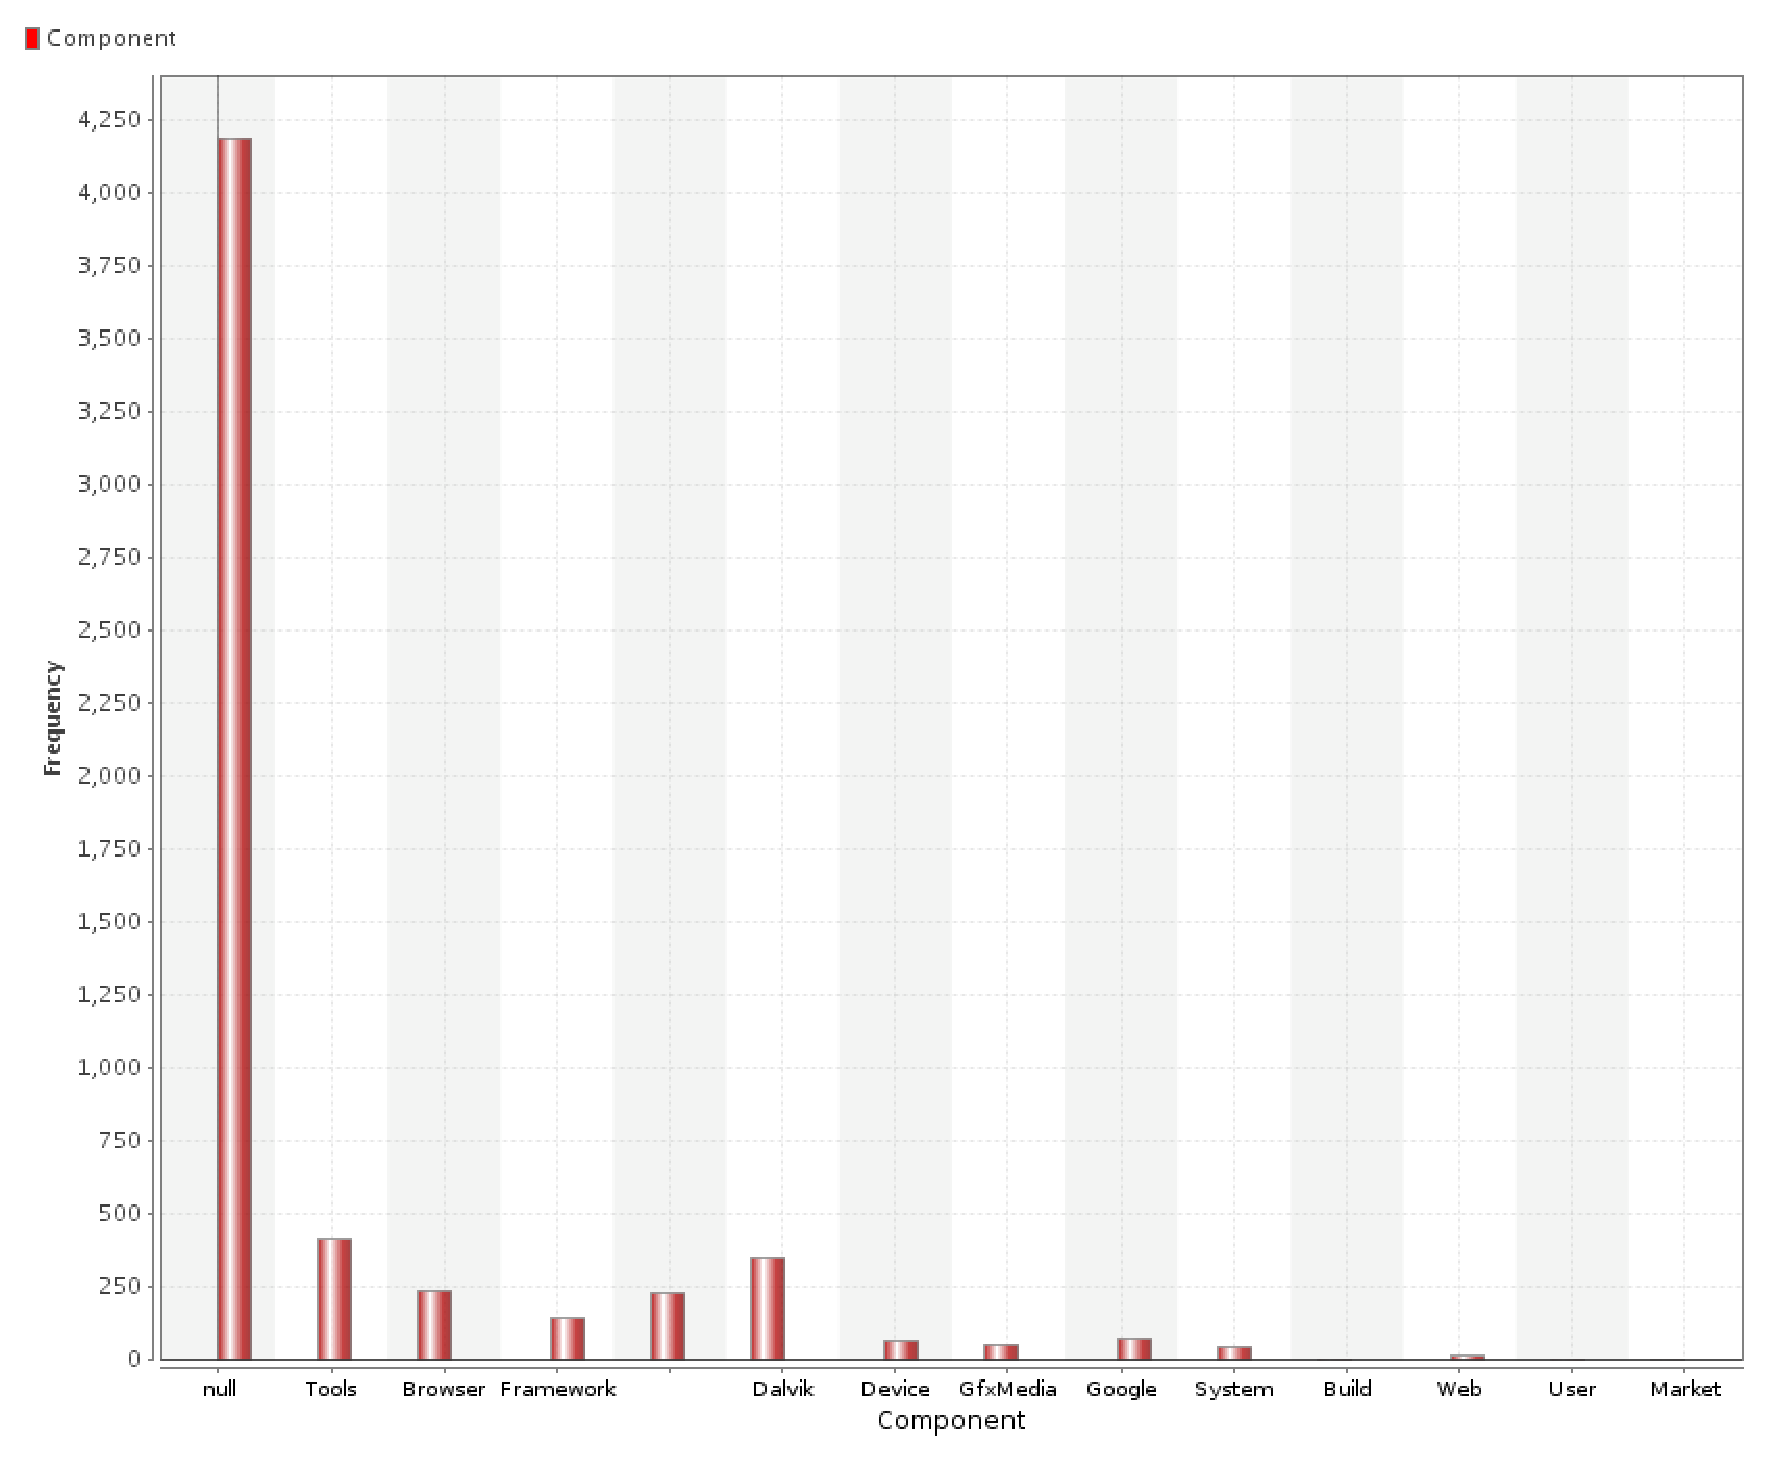
\includegraphics[scale=0.5]{hist-component}
\caption{\label{fig:component}Component distribution}
\end{center}
\end{figure}

\subsection*{Attributes used} % (fold)
\label{sub:Attributes used}
After inspecting the available data, we came to the conclusion that only title and description should be used to determine the component since they describe the bug but other properties are just metadata. The outcome of the classifier should be the component name that this bug affects.

\subsection*{Training and classes} % (fold)
\label{sub:Training and classes}
We need training data which should already be classified. Only the bugs which already had a component label assigned to them were chosen as the training data for data mining because the bugs with a component assigned to them are already classified and we didn't have to do it manually. There are about 10 different components used in the data, for example, Dalvik, System, Browser, Applications.
In the training there are a lot of missing labels as you can see in the  Figure~\ref{fig:component}. In our measurements I consider only the data with not null values.

The graphical representation of the processes of this data mining task can be seen in the following screenshot of Rapid Miner.


\subsection*{Text processing} % (fold)
\label{sub:Text processing}
Classifiers we used (k-NN, SVM and Decision Trees) can not work meaningfully with text directly, so it was necessary to preprocess text. The vector representation was choosen, because {\it SVM} and {\it k-NN} are designed for this representation and {\it Decision Trees} can be easily adjusted.

So title and description values were transformed into lower case
and then tokenized. Firstly, using non letters as delimiters and
secondly just the white space delimiters. Because of the
specific programming domain, simple white space separators were
more successful. Let us take example from the description
attribute. The tokenizer had to parse {\bf {\it
android.os.SystemClock.uptimeMillis()}}. According non letters
tokenizer the example will be parsed into {\bf {\it android}},
{\bf {\it os}}, {\bf {\it SystemClock}} etc., which divided into
several uncorrelated words. My hope had been that keeping the
words together will allow the classifiers discover the meaning
of the whole phrase. Unfortunately, I discovered that in general
the precision were improved only around $2\%$. I tried to
improved the performance by stemming, but I was not able to
observe any significant difference.

After tokenisation the word vectors were generated by using TF-IDF, binary term occurrences and term frequency.
In our example, one document was title and description of a bug.
The vectors consist of TF-IDF respectively binary term occurrences or term frequency values for one of all tokens and its values for the document.

After vector generation I selected first 1000 most significant words from the vectors and pass them to the classifier.

\begin{figure}
\begin{center} 
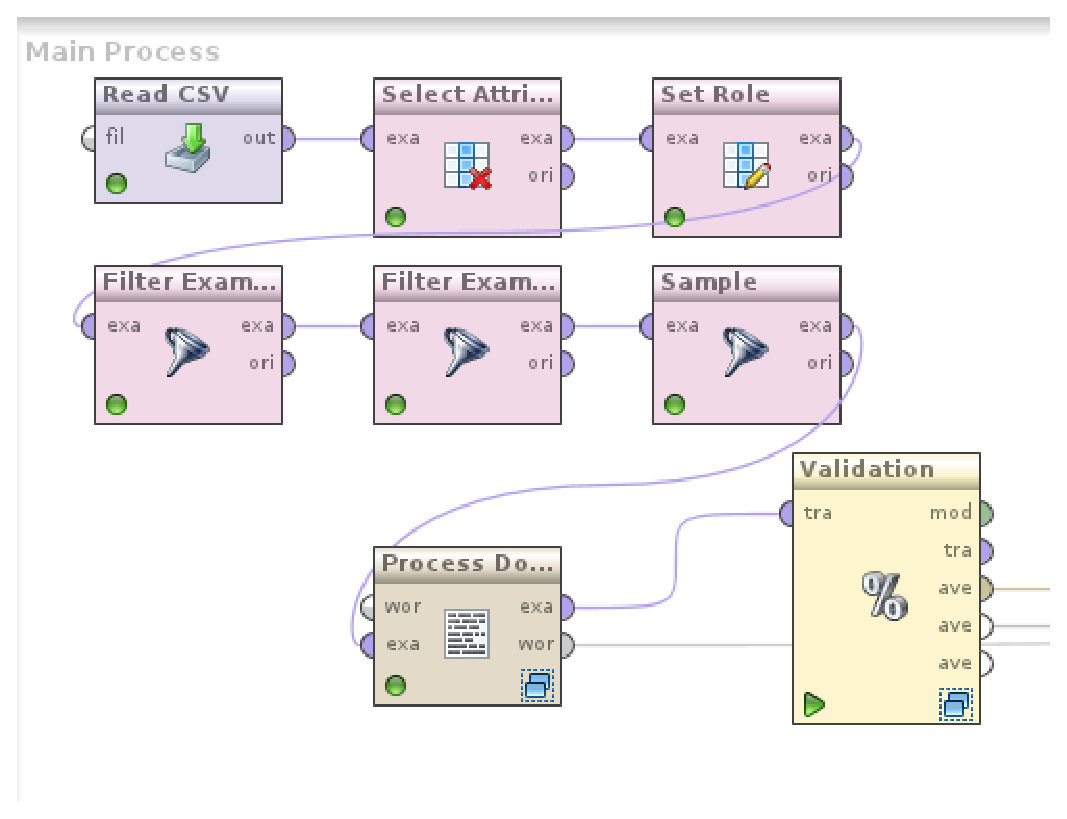
\includegraphics[scale=0.5]{rapidminer-process}
\caption{Process description: Process Document contains(tokenization, vectorisation, stemming), Validation contains(training, testing, performance measurement)}
\end{center}
\end{figure}
As general I can see that TF-IDF allows the classifiers best precision, term frequency is also usable alternative, but term occurrences performs the worst.
However, the performance heavily depends on the classifiers.
In the Figure~\ref{fig:vectors} you can see the comparison. 
I measured the decrease of performance from results of 10 experiments on 500 sample size.
I guess that {\it Decision Trees} are not influenced so strongly by change of the vector generation
technique, because they can not use TF-IDF properly and gives poorer result with TF-IDF.
It is worth to note, that despise the bigger decrease of successful rate by {\it 30-NN} and {\it SVM},
the overall performance order among {\it 30-NN}, {\it SVM} and {\it Decision Trees} remained the same.
\begin{figure}
\begin{center}
\begin{tabular}{|c|c|c|c|}
\hline
Classifier/Method     & 30-NN  & SVM &  Decision Tree   \\
Term Frequency        & 6\%    & 5\% &    3\%  \\
Term Occurrence       & 13\%   & 10\% &   5\%  \\
\hline
\end{tabular}
\caption{\label{fig:vectors} The decrease of performance of term frequency and binary term occurrence compare to TF-IDF}
\end{center}
\end{figure}

\subsection*{Performance} % (fold)
\label{sub:Performance}
 After the data was pre-processed, we chose various classifying algorithms that were learned about in class and compared their accuracy. Accuracy is used to assess the performance of classifiers. Because of lack of time and high amount of combination among experiments 5-fold cross validation was used instead of 10-fold cross validation. Also I reduced the sample size of data because it would take too much time to the classifiers to run on our desktop computers.

The overall performance was not improved much as you can see in Figure~\ref{fig:performance}

\begin{figure}
\begin{center}
\begin{tabular}{|c|c|c|c|c|}
\hline
Type     &       Algorithm    & Size &   Accuracy 1 & Accuracy 2  \\ \hline
\hline
Decision Trees & Weka J48      &   500  &       44.80\%   &    46.5\% \\
                              &&  1000  &      45.50\%  &    47.8\%\\
Decision Trees & Weka LAD-Tree &   500  &      39.80\%  &    41.6\%\\

Lazy Classifiers & 15-NN &   500  &      45.40\% &    43.4\% \\
                              &&  1000  &      49.70\%  &    50.7\%\\
                              &&  2000  &      55.90\%  &    54.8\%\\
 
Lazy Classifiers & 30-NN  &   500  &      45.10\%  &    46.2\%\\
                              &&  1000  &      49.00\%  &    49.9\%\\
                              &&  2000  &      54.40\%  &    55.3\%\\


SVM & Weka SMO &   500  &      41.40\% &      42.5\% \\
                                     &&  1000  &      47.20\% &      48.2\% \\
\hline
\end{tabular}
\caption{\label{fig:performance} Overall small improvements. Used TF-IDF, new tokenization, 800 vectors size}
\end{center}
\end{figure}


% section Classification (end)

